\documentclass{article}
\usepackage{geometry}
\geometry{a4paper, margin=1in}
\usepackage{graphicx}
\usepackage{listings}
\usepackage{xcolor}
\usepackage[utf8]{inputenc}

\lstset{
    basicstyle=\ttfamily\small,
    breaklines=true,
    frame=single,
    language=C,
    keywordstyle=\color{blue},
    commentstyle=\color{green!50!black},
    stringstyle=\color{red}
}

\begin{document}

\title{Operating Systems Lab Assignment: Concurrency with Semaphores, Critical Sections, and Monitor Locks}
\author{adam white}
\date{\today}
\maketitle

\section{Introduction}
This lab had six programs that use threads. Each one uses semaphores, mutexes, or condition variables so the threads don't mess up the data they share.

\section{Exercise 1: Producer-Consumer in C}
\lstinputlisting{producer_consumer.c}
\textbf{Explanation}: The program uses two semaphores and a mutex. empty starts at 5 and keeps track of how many open spots are in the buffer, and full starts at 0 and keeps track of how many items are in it. Before the producer adds something it waits on empty, and when it's done it posts full. The consumer does the opposite. The mutex is locked while a thread is changing the buffer so both of them can't be in there at once.

\textbf{Analysis}: Since the producer sleeps for 1 second and the consumer sleeps for 2, the producer gets ahead. By the end the producer was done and the consumer was still taking out the last few items. Everything came out in the same order it went in. If the semaphores weren't there, the producer could write over items that hadn't been read yet and the consumer could read from an empty spot. Taking out the mutex would let both threads change the buffer at the same time.

\begin{figure}[h]
    \centering
    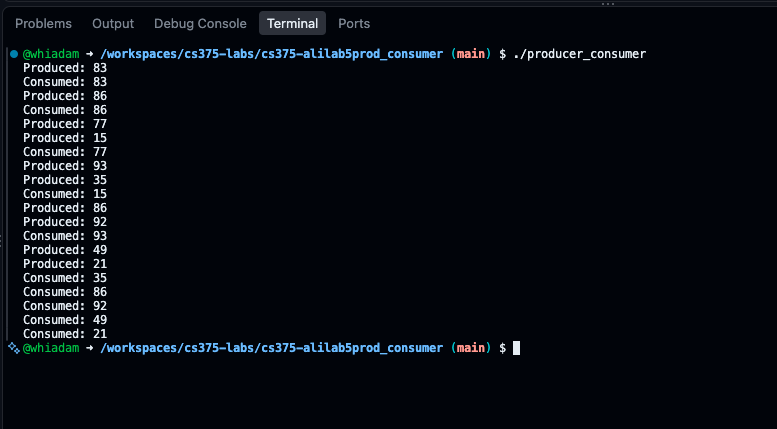
\includegraphics[width=\textwidth]{exercise1_screenshot.png}
    \caption{Compilation and execution of producer\_consumer.c}
\end{figure}

\section{Exercise 2: Bank Account Simulation in C++}
\lstinputlisting[language=C++]{bank_account.cpp}
\textbf{Explanation}: Both deposit and withdraw lock the mutex first, so only one thread can change the balance at a time. withdraw uses cv.wait to wait until there's enough money. When someone deposits, notify\_all wakes up anyone who was waiting so they can check the balance again.

\textbf{Analysis}: Five threads each deposit 100 and then withdraw 50. The balance went up to 600 and ended at 350, which is right since 100 + 500 - 250 = 350. None of the threads had to wait in this run because there was always more than 50 in the account. The wait is there so the balance can't go negative if a withdraw asks for more than what's there. Without the lock, two threads could read the same balance at once and one of the updates would get lost.

\begin{figure}[h]
    \centering
    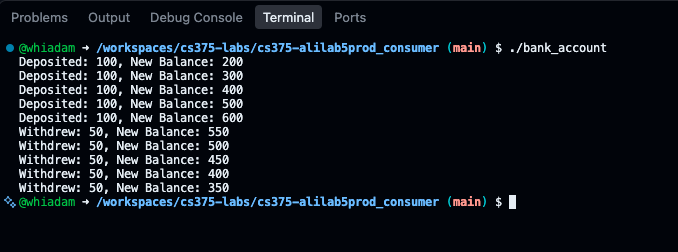
\includegraphics[width=\textwidth]{exercise2_screenshot.png}
    \caption{Compilation and execution of bank\_account.cpp}
\end{figure}

\section{Exercise 3: Reader-Writer Problem in C}
\lstinputlisting{reader_writer.c}
\textbf{Explanation}: rw\_mutex controls access to the shared data, and mutex just protects reader\_count. The first reader to come in waits on rw\_mutex, which locks out the writers, and the last reader to leave posts it. A writer has to get rw\_mutex by itself, so when a writer is in, nobody else is.

\textbf{Analysis}: This setup gives readers priority. In my output all three readers read 0 at the same time, then the two writers went one after the other and wrote 1 and 2. The downside is that if readers kept coming in nonstop, a writer could end up waiting forever. Without the semaphores a reader could see the data while it's being changed, and two writers doing shared\_data++ at once could lose an update.

\begin{figure}[h]
    \centering
    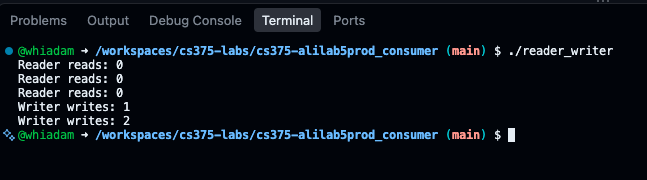
\includegraphics[width=\textwidth]{exercise3_screenshot.png}
    \caption{Compilation and execution of reader\_writer.c}
\end{figure}

\section{Exercise 4: Dining Philosophers in C++}
\lstinputlisting[language=C++]{dining_philosophers.cpp}
\textbf{Explanation}: Each fork is a mutex, and a philosopher has to lock two of them to eat. If all five grabbed their left fork at the same time, they would all be stuck waiting for the right one. The code fixes this by having the last philosopher swap the order, so every philosopher picks up the lower numbered fork first. That way the waiting can't go all the way around the table, so there's no deadlock.

\textbf{Analysis}: Each philosopher ate 3 times, so there were 15 lines. In my run the order was 1, 3, 0, 2, 4 every round. Two neighbors never ate at the same time since they share a fork. If the swap was taken out, the program could freeze with everyone holding one fork.

\begin{figure}[h]
    \centering
    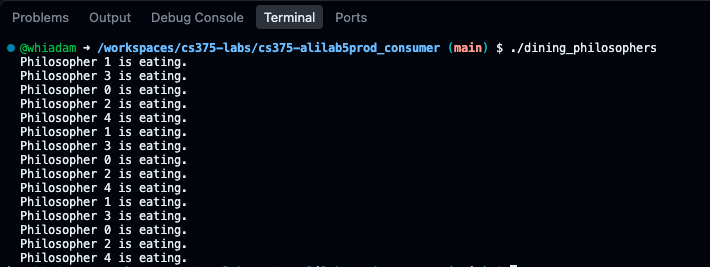
\includegraphics[width=\textwidth]{exercise4_screenshot.png}
    \caption{Compilation and execution of dining\_philosophers.cpp}
\end{figure}

\section{Exercise 5: Sleeping Barber Problem in C}
\lstinputlisting{sleeping_barber.c}
\textbf{Explanation}: There are three semaphores. customers counts how many people are waiting, and the barber sleeps on it when nobody is there. chairs starts at 3 and counts the open chairs. barber is how the barber tells a customer the haircut is done. When a customer shows up it tries to take a chair with sem\_trywait, and if there isn't one it just leaves. If it gets a chair, it posts customers to wake up the barber and then waits on barber. The mutex keeps two customers from grabbing chairs at the same time.

\textbf{Analysis}: A new customer shows up every second and each haircut takes 2 seconds, but 3 chairs was enough room and all five customers got haircuts. The barber thread is an infinite loop, so it never actually stops. The program still ends because main returns after all the customers finish. With no chairs semaphore, there would be no limit on how many customers could wait.

\begin{figure}[h]
    \centering
    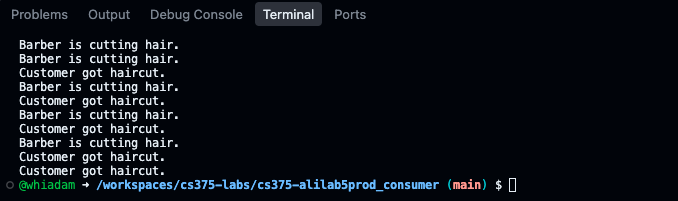
\includegraphics[width=\textwidth]{exercise5_screenshot.png}
    \caption{Compilation and execution of sleeping\_barber.c}
\end{figure}

\section{Exercise 6: Bounded Buffer with Condition Variables in C++}
\lstinputlisting[language=C++]{bounded_buffer.cpp}
\textbf{Explanation}: This is the same producer and consumer problem but with a mutex and two condition variables. The producer waits on not\_full until the queue has room, adds an item, and calls notify\_one on not\_empty. The consumer waits on not\_empty until there's something in the queue, takes it, and notifies not\_full. While a thread is waiting the lock gets released, so the other thread can still run.

\textbf{Analysis}: My output was exactly the same as Exercise 1, which makes sense because the sleep times are the same and rand() isn't seeded. The difference is how the buffer gets tracked. In Exercise 1 the semaphores hold the counts, and here the condition variables just check the actual size of the queue. I think this version is easier to read since the condition is written right in the code. The one thing that's harder is that you have to hold the lock to wait. For something that's just counting, semaphores are simpler.

\begin{figure}[h]
    \centering
    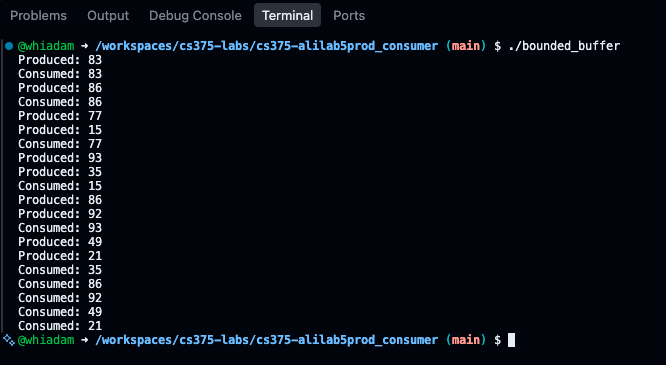
\includegraphics[width=\textwidth]{exercise6_screenshot.png}
    \caption{Compilation and execution of bounded\_buffer.cpp}
\end{figure}

\end{document}
